\documentclass{article}

\usepackage[margin=0.5in]{geometry}
\usepackage[inter-unit-product=\cdot,per-mode=symbol]{siunitx}
\usepackage{float}
\usepackage{amsmath}
\usepackage{vwcol}
\usepackage{multicol}
\usepackage{graphicx}
\usepackage{caption, copyrightbox}
\captionsetup{justification=centering, labelfont=sc, labelsep=endash}

\begin{document}
\section{Newton's laws of motion}
\subsection{Newton's first law of motion}
\begin{multicols}{2}
A body continues in its state of rest, or of uniform motion in a straight line, unless compelled to change that state by forces impressed upon it.
\vfill\null
\columnbreak
\begin{equation*}
	\boxed{\vec{p} = m\vec{V}}
\end{equation*}

\begin{align*}
\vec{p} &= \text{linear momentum vector (\si{\kilo\gram\meter\per\second})}\\
m &= \text{mass (\si{\kilo\gram})}\\
\vec{V} &= \text{velocity vector (\si{\meter\per\second})}\\
\end{align*}

\end{multicols}

\begin{multicols}{2}
\begin{equation*}
\boxed{\vec{H} = I\vec{\Omega}}
\end{equation*}

\begin{align*}
\vec{H} &= \text{angular momentum vector (\si{\kilo\gram\meter\squared\per\second})}\\
I &= \text{moment of inertia (\si{\kilo\gram\meter\squared})}\\
\vec{\Omega} &= \text{angular velocity vector (\si{\radian\per\second})}\\
\end{align*}

\vfill\null
\columnbreak

\begin{equation*}
\boxed{\vec{H} = \vec{R} \times m\vec{V}}
\end{equation*}

\begin{align*}
\vec{H} &= \text{angular momentum vector (\si{\kilo\gram\meter\squared\per\second})}\\
\vec{R} &= \text{position (\si{\meter})}\\
m &= \text{mass (\si{\kilo\gram})}\\
\vec{V} &= \text{velocity vector (\si{\meter\per\second})}\\
\end{align*}
\vfill\null
\end{multicols}

\subsection{Newton's second law of motion}
\begin{multicols}{2}
	The time rate of change of an object's momenutm equals the applied force.
	\vfill\null
	\columnbreak
	\begin{equation*}
	\boxed{\vec{F} = m\vec{a}}
	\end{equation*}
	
	\begin{align*}
	\vec{F} &= \text{force vector (\si{\kilo\gram\meter\per\second\squared = \newton})}\\
	m &= \text{mass (\si{\kilo\gram})}\\
	\vec{a} &= \text{acceleration  (\si{\meter\per\second\squared})}\\
	\end{align*}
	
\end{multicols}

\subsection{Newton's third law of motion}
When body A exerts a force on body B, body B will exert an equal, but opposite, force on body A

\section{Newton's laws of universal gravitation}
\begin{multicols}{3}

	\begin{equation*}
	\boxed{F_{g} = \dfrac{Gm_{1}m_{2}}{R^{2}}}
	\end{equation*}
	\vfill\null
	\columnbreak
	\begin{align*}
	F_{g} &= \text{force due to gravity (\si{\newton})}\\
	G &= \text{universal gravitational constant} \approx
	  6.674 \times 10^{-11}\,\si{\newton \meter\squared\per\kilo\gram\squared}\\
	m_{1}, m_{2} &= \text{masses of two bodies  (\si{\kilo\gram})}\\
	R &= \text{distance between the two bodies  (\si{\meter})}\\
	\end{align*}
\end{multicols}
\begin{multicols}{3}
	\begin{equation*}
	\boxed{a_{g} = \dfrac{\mu_{Earth}}{R^{2}}}
	\end{equation*}
	\vfill\null
	\columnbreak
	\begin{align*}
	a_{g} &= \text{acceleration due to gravity (\si{\meter\per\second\squared})}\\
	\mu_{Earth} &\equiv G\,m_{Earth} \approx 3.986 \times 10^{14} \, \si{\meter\cubed\per\second\squared}\\
	R &= \text{distance between the two bodies  (\si{\meter})}\\
	\end{align*}

	\vfill\null
\end{multicols}

\section{Laws of conservation}
\subsection{Conservation of momentum}
In the absence of outside forces, linear and angular momentum are conserved.

\subsection{Energy}
\begin{multicols}{3}
	\begin{equation*}
	\boxed{E = KE + PE}
	\end{equation*}

	\begin{align*}
	E &= \text{total mech. energy (\si{\kilo\gram\,\meter\squared\per\second\squared)}}\\
	KE &= \text{kinetic energy (\si{\kilo\gram\,\meter\squared\per\second\squared)}}\\
	PE &= \text{potential energy (\si{\kilo\gram\,\meter\squared\per\second\squared)}}\\
	\end{align*}
	
	\vfill\null
	\columnbreak
	
	\begin{equation*}
	\boxed{PE = m\,a_{g}h}
	\end{equation*}
	
	\begin{align*}
	m &= \text{mass (\si{\kilo\gram})}\\
	a_{g} &= \text{acceleration due to gravity (\si{\meter\per\second\squared})}\\
	h &= \text{height above ref. point (\si{\meter})}\\
	\end{align*}
	\vfill\null
	\columnbreak
	
	\begin{equation*}
	\boxed{PE = -\dfrac{m\mu}{R}}
	\end{equation*}
	
	\begin{align*}
	m &= \text{spacecraft's mass (\si{\kilo\gram})}\\
	\mu &= \text{gravitational parameter (\si{\kilo\meter\cubed\per\second\squared})}\\
	R &= \text{distance from Earth's center (\si{\kilo\meter})}\\
	\end{align*}
	\vfill\null
\end{multicols}

\begin{multicols}{2}
	\begin{equation*}
	\boxed{KE = \dfrac{1}{2} m V^{2}}
	\end{equation*}
	
	\begin{align*}
	KE &= \text{kinetic energy (\si{\kilo\gram\,\meter\squared\per\second\squared)}}\\
	m &= \text{mass (\si{\kilo\gram})}\\
	V &= \text{velocity (\si{\kilo\meter\per\second}})\\
	\end{align*}
	
	\vfill\null
	\columnbreak
	
	\begin{equation*}
	\boxed{E = \dfrac{1}{2} m V^{2} - \dfrac{m\mu}{R}}
	\end{equation*}
	
	\begin{align*}
	E &= \text{total mech. energy (\si{\kilo\gram\,\meter\squared\per\second\squared)}}\\
	m &= \text{mass (\si{\kilo\gram})}\\
	V &= \text{velocity (\si{\kilo\meter\per\second}})\\
	\mu &= \text{gravitational parameter (\si{\kilo\meter\cubed\per\second\squared})}\\
	R &= \text{position (\si{\kilo\meter})}\\
	\end{align*}
	\vfill\null
\end{multicols}

\section{The restricted two-body problem}
\subsection{Coordinate systems}

\begin{figure*}[!h]
	\centering
	\copyrightbox[r]{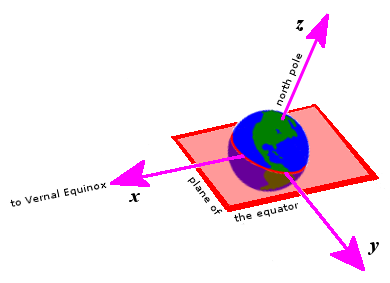
\includegraphics[width=0.7\linewidth]{img/Ra_and_dec_rectangular}}{\textcopyright By Tfr000 (talk) 19:24, 23 April 2012 (UTC) - Own work, CC BY-SA 3.0, https://commons.wikimedia.org/w/index.php?curid=19193590}
	\caption{Geocentric equatorial coordinates. The origin is the centre of the Earth. The fundamental plane is the plane of the Earth's equator. The primary direction (the x axis) is the vernal equinox. A right-handed convention specifies a y axis 90° to the east in the fundamental plane; the z axis is the north polar axis. The reference frame does not rotate with the Earth, rather, the Earth rotates around the z axis.}
	\label{fig:coordinate_system}
\end{figure*}


A coordinate system (figure \ref{fig:coordinate_system}) is:
\begin{itemize}
	\item \textbf{an origin}
	\item \textbf{a fundamental plane}, containing two axes, and the perpendicular to it
	\item \textbf{a principal direction} within the plane
	\item \textbf{the third axis} using the right-hand rule
\end{itemize}

\subsection{Equation of motion}
\begin{equation*}
\boxed{\ddot{\vec{R}} + \dfrac{\mu}{R^{2}} \dfrac{\vec{R}}{R} = 0}
\end{equation*}

\begin{align*}
\ddot{\vec{R}} &= \text{spacecraft's acceleration (\si{\kilo\meter\per\second\squared})}\\
\mu &= \text{gravitational parameter (\si{\kilo\meter\cubed\per\second\squared})}\\
\vec{R} &= \text{spacecraft's position vector (\si{\kilo\meter})}\\
R &= \text{magnitude of the spacecraft's position vector (\si{\kilo\meter})}\\
\end{align*}

\subsection{Orbital geometry}

\begin{minipage}{0.6\textwidth}
	\begin{figure}[H]
		\centering
		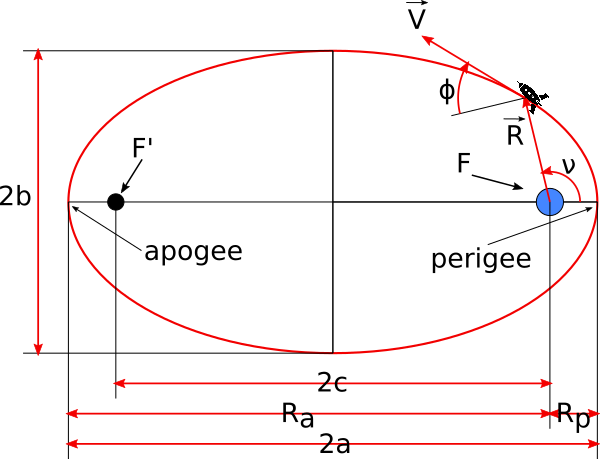
\includegraphics[width=0.9\linewidth]{img/ellipse}
		\caption{Geometry of an elliptical orbit}
		\label{fig:coordinate_system}
	\end{figure}
\end{minipage} \hfill
\begin{minipage}{0.35\textwidth}
	\begin{align*}
	\vec{R} &= \text{spacecraft's position vector}\\
	\vec{V} &= \text{spacecraft's velocity vector}\\
	F and F' &= \text{primary and vacant foci}\\
	R_{p} &= \text{radius of perigee}\\
	R_{a} &= \text{radius of apogee}\\
	2a &= \text{major axis}\\
	2b &= \text{minor axis}\\
	2c &= \text{distance between the foci}\\
	a &= \text{semimajor axis}\\
	b &= \text{semiminor axis}\\
	\nu &= \text{true anomaly}\\
	\phi &= \text{flight-path angle}\\
	\end{align*}
\end{minipage}

\end{document}
